\documentclass[a4paper]{ltjsarticle}
\usepackage{xfakebold,tcolorbox,amsmath,amssymb,graphicx,ascmac,fancybox,framed,tikz,comment,calc,amsthm,bm,enumitem}
\tcbuselibrary{breakable, skins, theorems}
\usetikzlibrary{positioning, intersections, calc, arrows.meta,math}
\usepackage[top=11truemm,left=20truemm,right=15truemm,bottom=23truemm]{geometry}

% \white :計算用余白の挟み込み
\newcommand{\white}{\newgeometry{top=20truemm}\leavevmode
\begin{center}
    \noindent(\,計　算　用　余　白\,)
\end{center}}
% \exc[サイズ]{数値} :a\exc{b}でa^b, 指数に指数を載せる時に使用　数式環境内ではサイズ0.95
\newcommand{\exc}[2][0.75]{^{\textstyle\scalebox{#1}[#1]{\raise0.25ex\hbox{$#2$}}}}
% \exfrac[サイズ]{分母}{分子} :指数部分に分数を持ってくるときに使う．積分範囲などに使う場合サイズ0.75~0.8を推奨
\newcommand{\exfrac}[3][0.90]{\tfrac{\lower0.1ex\hbox{\scalebox{#1}[#1]{$#2$}}}{\raise0.3ex\hbox{\scalebox{#1}[#1]{$#3$\rule{0pt}{7.5pt}}}}}
% \dint[文字サイズ]{下付}{上付} :インテグラルのdisplay省略、積分範囲の表示サイズを変更、
\newcommand{\dint}[3][0.75]{\displaystyle\int_{\scalebox{#1}[#1]{$#2$}}^{\scalebox{#1}[#1]{$#3$}}}
% \dsqrt[n乗根]{中身}　:√を重ねる時用
\newcommand{\dsqrt}[2][]{\displaystyle\sqrt[\raise0ex\hbox{{\scalebox{0.625}[0.625]{$#1$}}}]{#2}}
% \dlim{下に付けるヤツ} :文字サイズ変更に適用させたlim
\newcommand{\dlim}[1]{\raise0.3ex\hbox{\scalebox{1.04}{${\normalsize \displaystyle\lim_{#1}}$}}\,}
% \cmb{n}{r}  \prm{n}{r}　: nCr nPr
\def\cmb#1#2{_{#1}\mathrm{C}_{#2}}\def\prm#1#2{_{#1}\mathrm{P}_{#2}}
% \w :(n)の後の空白用
\def\w{\;\;\;}\def\spw{\;\;}
% \hs \vs \vhs  :未使用
\def\hs{\hspace{1.38cm}}\def\vs{\vspace{-2mm}\\[1mm]}\def\vhs{\vs\hs}
\def\mrm{\mathrm}
\def\ve{\overrightarrow}
% 表紙のページ番号を省略
\setcounter{page}{0}
\usepackage{setspace}
\setstretch{1.4}
% ----[設定]----------------------------
    % setting.texから設定を調整すること
    % 注意事項
    % 0:一般，1:条件を伴う，2:選択を伴う，3:どっちも伴う
        \newcommand{\precaution}{2}
    % 問題の個数
        \newcommand{\amountq}{4}
    % precautionが1,3の場合: 必答[req], 選択[select], 合計点[の条件]
        \newcommand{\scorereq}{80}
        \newcommand{\scoreselect}{80}
        \newcommand{\scoretotal}{180}
    % precautionが2,3の場合: 必答[req]，選択[select]の問題番号先頭[h]と末尾[e]
        \newcommand{\hreq}{1}
        \newcommand{\ereq}{4}
        \newcommand{\hselect}{5}
        \newcommand{\eselect}{8}
        \newcommand{\amountsel}{4}
    % 実施日 令和exey\exem月\exed日\exew曜日
        \newcommand{\exey}{8}
        \newcommand{\exem}{5}
        \newcommand{\exed}{12}
        \newcommand{\exew}{木}

% 表紙設定
    % \condyear: 何年度の試験か，\condmonth: 何月の試験か
        \newcommand{\condyear}{2026}
        \newcommand{\condmonth}{4}
    % \examtime: 試験時間，\maxscore: 点数の最高値
        \newcommand{\examtime}{100}
        \newcommand{\maxscore}{80}
% -------------------------------
\setcounter{page}{1}

% ----[ここから本文]---------------------
\begin{document}

% ----[表紙]----------------------------
%\fontsize{11truept}{11truept}\selectfont
\setlist{parsep=0ex, itemsep=1ex, leftmargin=1.5cm}
\thispagestyle{empty}
    % 受験番号タイトル設定日付
    \begin{center}
        % 氏名
        \leavevmode\hfill\scalebox{0.8}{
        \begin{tabular}{|l|r|} \hline
            % LuaLaTeXする前だけどなんか真ん中持ってけないからごり押し
            % 今度資料集めてきて形式直す、受験番号2行かもみんあ
            \lower1.5ex\hbox{　\hspace{-0.25cm}}{\large 受\;験\;番\;号}\raise1.5ex\hbox{　\hspace{-0.25cm}} & \hspace{6cm} \\ \hline
        \end{tabular}}\leavevmode\\[0mm]\vspace{-0.05cm}　\hfill\scalebox{0.8}{
        \begin{tabular}{|l|r|} \hline
            \lower1.5ex\hbox{　\hspace{-0.15cm}}{\large 氏\;名}\raise1.5ex\hbox{　\hspace{-0.15cm}} & \hspace{6.814cm} \\ \hline
        \end{tabular}}\\[15mm]
        \scalebox{1.4}{ ${{\setBold[0.01]\condyear\;年度　\condmonth\;月実施　模擬試験\unsetBold}}$ }
        \\[7mm]
        　　　　\scalebox{1.3}{{\Huge $数\spw \spw \spw 学$}}　　　
        \\[2mm]
        {\large 　(\;\examtime\;分　　\maxscore\;点\;)}
    \end{center}
　\\[15mm]
    \hfill \scalebox{1.5}{{\Large  令和\;$\exey$\;年　\;$\exem$\;月\;$\exed$\;日\;(\exew)}}
　\\[2mm]
    \begin{framed}
        {\large 付属の解答用紙を使用する際は指定された枠に問題の解答を記述し提出すること．使用しな}\\[1.5mm]
        {\large い場合はA4，もしくはB5サイズの白紙に解答を問題番号及び小問番号等すべてが明確にわか}\\[1.5mm]
        {\large るように記述し提出すること．}
        　\\[-3mm]
    \end{framed}
\leavevmode\\[2mm]
    % 注意事項
        \leavevmode
        \centerline{{\Large 　\;\;$\textgt{{\mdseries 注　意　事　項}}$\;\;　}}
        \\[0mm]
        \fontsize{12}{12}\selectfont
\begin{enumerate}[parsep=0ex, itemsep=1.5ex, leftmargin=0.6cm]
\input{pre/precautions/\precaution.tex}
\end{enumerate}


\vfill


\setlist{parsep=0ex, itemsep=1ex, leftmargin=2.5cm}

% 本文用設定に変更、文字サイズエラーは無視
\newgeometry{left=15truemm,right=20truemm,top=25truemm}\fontsize{14truept}{14truept}\selectfont
\newgeometry{left=20truemm,right=20truemm,top=30truemm}\noindent
\scalebox{2}{\fbox{1}}　
\\[5mm]
　次の式を因数分解しなさい。\\[-5mm]
\begin{enumerate}
    \item[(1)　]$xy+x^2$
    \item[(2)　]$x^2-x-2$
    \item[(3)　]$4x^2-6x+9$
    \item[(4)　]$x^4-16$ \latex
\end{enumerate}\leavevmode\\[-5mm]
　次の方程式を解きなさい。\\[-5mm]
\begin{enumerate}
    \item[(5)　]$3x-2=-8$
    \item[(6)　]$\dfrac{1}{3}(x-2)=\dfrac{3}{2}(1-x)$
    \item[(7)　]$x^2-3x+2=0$
    \item[(8)　]$2x^2-5x+3=0$
    \item[(9)　]$x^2+4x+1=0$ 
\end{enumerate}\leavevmode\\[-5mm]
　次の関数の値域を求めなさい。\\[-5mm]
\begin{enumerate}
    \item[(10)　]$y=2x-1$　$(-1<x<1)$
    \item[(11)　]$y=-x+3$　$(0<x)$
    \item[(12)　]$y=2x^2$　$(2<x<5)$
    \item[(13)　]$y=x^2$　$(-1<x<2)$
\end{enumerate}

\newpage\noindent
\scalebox{2}{\fbox{2}}　\\[5mm]\indent
　以下の$3$つのグラフの交点を求め、例にならって図示しなさい。
\begin{enumerate}
    \item[]$y=2x^2$，$y=-x^2$，$y=x$
\end{enumerate}
{\Large 例}\\
　\scalebox{.4}{
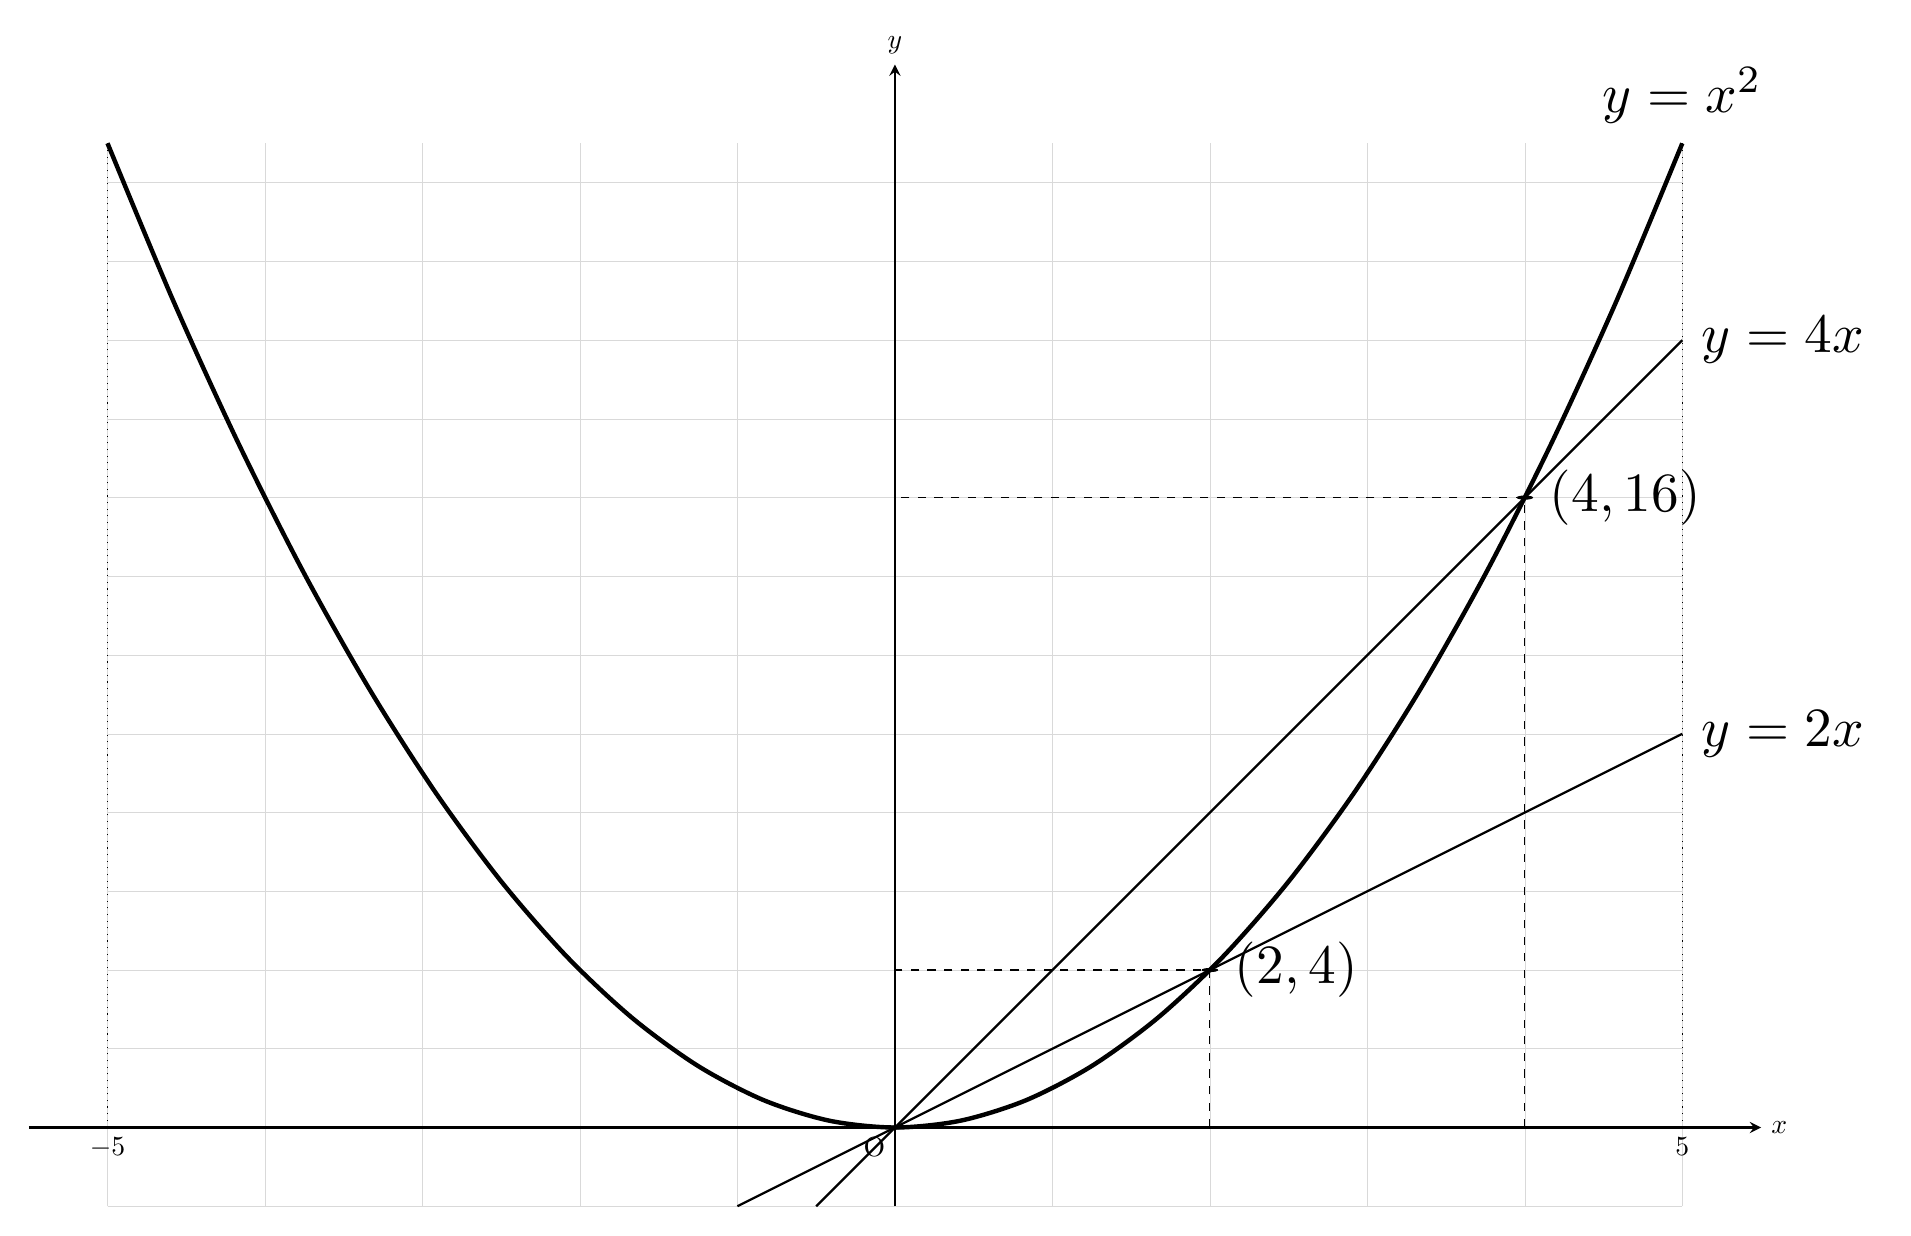
\begin{tikzpicture}[>=stealth, xscale=2, yscale=0.5]
    % グリッド
    \draw[help lines, black!15, xstep=1, ystep=2] (-5,-2) grid (5,25);

    % 座標軸
    \draw[->, thick] (-5.5,0) -- (5.5,0) node[right] {$x$};
    \draw[->, thick] (0,-2) -- (0,27) node[above] {$y$};
    \node[below left] at (0,0) {O};

    % グラフの描画
    \draw[domain=-5:5, smooth, variable=\x, black, ultra thick] plot ({\x}, {\x*\x});
    \draw[domain=-0.5:5, smooth, variable=\x, black, thick] plot ({\x}, {4*\x});
    \draw[domain=-1:5, smooth, variable=\x, black, thick] plot ({\x}, {2*\x});

    % 交点のプロット
    \fill (0,0) circle (1.5pt); % xscaleの影響で楕円にならんよう小さめに
    
    % (2,4)
    \fill (2,4) circle (1.5pt);
    \draw[dashed] (2,0) -- (2,4) -- (0,4);
    \node[right, xshift=2pt, scale=2] at (2,4) {$(2,4)$};

    % (4,16)
    \fill (4,16) circle (1.5pt);
    \draw[dashed] (4,0) -- (4,16) -- (0,16);
    \node[right, xshift=2pt, scale=2] at (4,16) {$(4,16)$};

    % 式のラベル（横に伸びた分、位置を調整）
    \node[black, scale=2, above] at (5, 25) {$y=x^2$};
    \node[black, scale=2, anchor=west] at (5, 20) {$y=4x$};
    \node[black, scale=2, anchor=west] at (5, 10) {$y=2x$};

    % x=-5, 5 のガイド
    \draw[dotted] (-5,0) -- (-5,25);
    \draw[dotted] (5,0) -- (5,25);
    \node[below] at (-5,0) {$-5$};
    \node[below] at (5,0) {$5$};

\end{tikzpicture}}
\vfill\rightline{{\LARGE 問題は以上である\w}}\leavevmode\\[6mm]


\end{document}